%%%%%%%%%%%%%%%%%%%%%%%%%%%%%%%%%%%%%%%%%%%%%%%%%%%%%%%%%%%%%%%%%%%%%%%%%%%%%%%
% Titel:   PA1 - Dokumentation
% Autor:   Nicola K�ser
% Datum:   28.10.2013
% Version: 0.1.0
%%%%%%%%%%%%%%%%%%%%%%%%%%%%%%%%%%%%%%%%%%%%%%%%%%%%%%%%%%%%%%%%%%%%%%%%%%%%%%%
% Versionshinweise und �nderungsprotokol:
%
%  v0.0.1  2013-10-14  Erste Formulierung in Microsoft Word, mit Konzentration
%                      auf den Inhalt, da das Dokument so bald wie m�glich in
%                      LaTeX umformatiert wird.
%  v0.0.2  2013-10-23  Inhalterweiterung
%  v0.1.0  2013-10-28  Konvertierung in LaTeX
%%%%%%%%%%%%%%%%%%%%%%%%%%%%%%%%%%%%%%%%%%%%%%%%%%%%%%%%%%%%%%%%%%%%%%%%%%%%%%%
\documentclass[version=last,fleqn,numbers=noenddot]{scrreprt}
	% version=first:    Ergebniss Kompatibel zu ersten Version;
	%         last:     Ergebniss entspricht den aktuellen Paketen;
	% fleqn:            Formeln linksb�ndig;
	% numbers=noenddot: Kapitelnummerierung ohne Punkt;
	%         enddot:   Kapitelnummerierung mit Punkt;
	% twoside:          Doppelseitiger Druck

% Dokumentangaben
\newcommand{\Titel}         {Eurobot 2014 Naherkennung}
\newcommand{\Uebertitel}    {Projektarbeit 1 - Dokumentation}
\newcommand{\AutorA}        {Nicola K\"aser}
\newcommand{\Dozent}        {M. Kucera}
\newcommand{\Datum}         {\today}
\newcommand{\Ort}           {Burgdorf}
\newcommand{\Version}       {0.1.0}



%%%%%%%%%%%%%%%%%%%%%%%%%%%%%%%%%%%%%%%%%%%%%%%%%%%%%%%%%%%%%%%%%%%%%%%%%%%%%%%
% Pakete
%%%%%%%%%%%%%%%%%%%%%%%%%%%%%%%%%%%%%%%%%%%%%%%%%%%%%%%%%%%%%%%%%%%%%%%%%%%%%%%
% Maximale Tiefe des Inhaltsverzeichnis und Tiefe der Verzeichnis�ffnung im PDF
\newcommand{\tocmaxdepth}   {2}
%%%%%%%%%%%%%%%%%%%%%%%%%%%%%%%%%%%%%%%%%%%%%%%%%%%%%%%%%%%%%%%%%%%%%%%%%%%%%%%
% Titel:   Bericht - Pakete
% Autor: Simon Grossenbacher  
% Datum:   27.09.2013
% Version: 1.0.0
%%%%%%%%%%%%%%%%%%%%%%%%%%%%%%%%%%%%%%%%%%%%%%%%%%%%%%%%%%%%%%%%%%%%%%%%%%%%%%%
%
%:::Change-Log:::
% Versionierung erfolgt auf folgende Gegebenheiten: -1. Release Versionen
%                                                   -2. Neue Kapitel
%                                                   -3. Fehlerkorrekturen
%
% 0.0.0       Erstellung der Datei
%
%:::Hinweis:::
% Indexerstellung: makeindex -s report.ist report.idx
%   Umlaute m�ssen separat behandelt werden!
%%%%%%%%%%%%%%%%%%%%%%%%%%%%%%%%%%%%%%%%%%%%%%%%%%%%%%%%%%%%%%%%%%%%%%%%%%%%%%%

%Sprach-Optionen
\usepackage[ngerman]{babel} %neue deutsche Rechtschreibung
\usepackage[T1]{fontenc}  %richtige Worttrennung
%\usepackage[applemac]{inputenc}                % Mac - load extended character set (ISO 8859-1)
%\usepackage[latin1]{inputenc}                   % Unix/Linux - load extended character set (ISO 8859-1)
\usepackage[ansinew]{inputenc}                 % Windows - load extended character set (ISO 8859-1)
%\usepackage[utf8]{inputenc}                    % UTF-8 encoding

%Zeilenabstand
\usepackage{setspace}

%Mehr Tabellenoptionen
\usepackage{tabularx}
\usepackage{longtable}

%Listen
\usepackage{enumitem}

%Besserer Flattersatz
\usepackage{ragged2e}

%Gleiten verhindern
\usepackage{float}
\usepackage{placeins}

%Z�hler per Seite resetten (z.B. Fussnoten-Index)
\usepackage{perpage}

%Ueberschriften anpassen
\usepackage{titlesec} 

%Farben
\usepackage{color}
\usepackage{colortbl} %F�r farbige Tabellen

%PDF zu Dokument hinzufuegen
\usepackage[final]{pdfpages}

%Grafiken verwalten
\usepackage{graphicx}
\usepackage[absolute]{textpos}

%Zeichnen
%\usepackage{pst-pdf}
%\usepackage{pst-all}

%Listnings verwalten
\usepackage{listings}

%Kopf- Fusszeile (Optionen m�ssen direkt �bergeben werden)
\usepackage[automark, %Automatisches aktualisieren der Chapter-Titel
%            headsepline,  %Linie Kopfzeile
%            footsepline,  %Linie fusszeilezeile
%            markuppercase,
            plainfootsepline  %Plain-Style auch mit Linie versehen
            ]{scrpage2}

%Flexible Argumente bei Funktionen
\usepackage{xargs}

%erweiterte Steuerfunktionen
\usepackage{ifthen}

%Index f�r Stichwortverzeichnis
\usepackage{makeidx}

%Index f�r Literaturverzeichnis
\usepackage[babel,german=quotes]{csquotes}
%\usepackage[backend=biber,style=numeric,defernumbers=true,sorting=nyt]{biblatex}
\usepackage[backend=bibtex,defernumbers=true]{biblatex}
\bibliography{bibliography}
\defbibheading{lit}{\section{Literatur}}
\defbibheading{pic}{\section{Abbildungen}}

%Zusaetzliche Symbole direkt im Text
\usepackage{textcomp}
\usepackage{amssymb}

%Einheit kontrolliert eingeben
\usepackage{units}

%dynamische Datumsausgabe
\usepackage[german]{isodate}

%Zusaetzlich Mathemtiksymbole
\usepackage{amsmath}
\usepackage{mathtools}

%Besser Handling von internen Countern und Berechnungen
\usepackage{calc}

%TODOs anbringen am Rand
\usepackage{todonotes}

%Hyperlinks (Muss das letzte geladene Paket sein)
\usepackage[bookmarks=true, %Verzeichnis generieren
            bookmarksopen=true, %Verzeichnis �ffnen
            bookmarksopenlevel=\tocmaxdepth, %Tiefe der Verzeichnis�ffnung
            unicode=false, %non-Latin Zeichen
            pdftoolbar=true, %PDF-Viewer Toolbar
            pdfmenubar=true, %PDF-Viewer Men�?
            pdffitwindow=true, %Fenster an Seite anpassen beim �ffnen
            pdftitle={\Titel}, %Titel
            %pdfauthor={\Autor1, \Autor2, \Autor3}, %Autor
            pdfsubject={\Uebertitel}, %Thema
%            pdfcreator={\Autor1, \Autor2, \Autor3}, %Ersteller des Dokuments
%            pdfproducer={\Autor1, \Autor2 \Autor3}, %Produzent des Dokuments
            pdfnewwindow=true, %Links in neuem Fenster
            colorlinks=true, %false: Boxen-Links; true: Farben-Links
            linkcolor=black, %Farbe von internen Links
            citecolor=black, %Farbe von Links zu Bibliography
            filecolor=magenta, %Farbe von Links zu Dateien
            urlcolor=blue %Farbe von externen Links
            ]{hyperref}
            
%Glossar/Abk�rzungsverzeichnis
\usepackage[acronym,makeindex]{glossaries}




%%%%%%%%%%%%%%%%%%%%%%%%%%%%%%%%%%%%%%%%%%%%%%%%%%%%%%%%%%%%%%%%%%%%%%%%%%%%%%%
% Optionen
%%%%%%%%%%%%%%%%%%%%%%%%%%%%%%%%%%%%%%%%%%%%%%%%%%%%%%%%%%%%%%%%%%%%%%%%%%%%%%%
% Flag ob ein Abbildungs- und Tabellenverzeichnis erstellt werden soll
\setnewboolean{createLists}     {true}
% Flag ob ein Stichwortverzeichnis erstellt werden soll
\setnewboolean{createIndex}     {true}
% Flag ob ein �bersichtsverzeichnis erstellt werden soll
\setnewboolean{createShorttoc}  {true}



%%%%%%%%%%%%%%%%%%%%%%%%%%%%%%%%%%%%%%%%%%%%%%%%%%%%%%%%%%%%%%%%%%%%%%%%%%%%%%%
% Funktionen
%%%%%%%%%%%%%%%%%%%%%%%%%%%%%%%%%%%%%%%%%%%%%%%%%%%%%%%%%%%%%%%%%%%%%%%%%%%%%%%
%%%%%%%%%%%%%%%%%%%%%%%%%%%%%%%%%%%%%%%%%%%%%%%%%%%%%%%%%%%%%%%%%%%%%%%%%%%%%%%
% Titel:   Bericht - Funktionen
% Autor:   Simon Grossenbacher
%          Nicola K�ser (v1.1.0)
% Datum:   27.09.2013
% Version: 1.1.0
%%%%%%%%%%%%%%%%%%%%%%%%%%%%%%%%%%%%%%%%%%%%%%%%%%%%%%%%%%%%%%%%%%%%%%%%%%%%%%%
%
%:::Change-Log:::
% Versionierung erfolgt auf folgende Gegebenheiten: -1. Release Versionen
%                                                   -2. Neue Kapitel
%                                                   -3. Fehlerkorrekturen
%
% 0.0.0       Erstellung der Datei
% 1.0.0       Release
% 1.1.0       Erg�nzungen
%
%:::Hinweis:::
% Indexerstellung: makeindex -s report.ist report.idx
%   Umlaute m�ssen separat behandelt werden!
%%%%%%%%%%%%%%%%%%%%%%%%%%%%%%%%%%%%%%%%%%%%%%%%%%%%%%%%%%%%%%%%%%%%%%%%%%%%%%%

%%%%%%%%%%%%%%%%%%%%%%%%%%%%%%%%%%%%%%%%%%%%%%%%%%%%%%%%%%%%%%%%%%%%%%%%%%%%%%%
% Text tiefstellen
% param #1 Text
%%%%%%%%%%%%%%%%%%%%%%%%%%%%%%%%%%%%%%%%%%%%%%%%%%%%%%%%%%%%%%%%%%%%%%%%%%%%%%%
\newcommand{\low}[1]{\textsubscript{#1}}



%%%%%%%%%%%%%%%%%%%%%%%%%%%%%%%%%%%%%%%%%%%%%%%%%%%%%%%%%%%%%%%%%%%%%%%%%%%%%%%
% Text hochstellen
% param #1 Text
%%%%%%%%%%%%%%%%%%%%%%%%%%%%%%%%%%%%%%%%%%%%%%%%%%%%%%%%%%%%%%%%%%%%%%%%%%%%%%%
\newcommand{\high}[1]{\textsuperscript{#1}}



%%%%%%%%%%%%%%%%%%%%%%%%%%%%%%%%%%%%%%%%%%%%%%%%%%%%%%%%%%%%%%%%%%%%%%%%%%%%%%%
% Schrift anpassen
% param #1 Schriftfamilie: ptm Times
%                          phv Helvetica
%                          pcr Courier
%                          pbk Bookman
%                          pag Avant Garde
%                          ppl Palatino
%                          pch Charter
%                          pnc New Century Schoolbook
%                          put Utopia
% param #2 Strichdicke/Zeichenbreite: b  bold
%                                     m  medium
% param #3 Schriftform: n   normal
%                       it  italic
%                       sl  slanted
%                       sc  small caps
%                       ui  upright italic
% note {\changefont{#1}{#2}{#3} Hallo Welt} Teilbereich aendern
%%%%%%%%%%%%%%%%%%%%%%%%%%%%%%%%%%%%%%%%%%%%%%%%%%%%%%%%%%%%%%%%%%%%%%%%%%%%%%%
\newcommand{\changefont}[3]{\fontfamily{#1} \fontseries{#2} \fontshape{#3} \selectfont}



%%%%%%%%%%%%%%%%%%%%%%%%%%%%%%%%%%%%%%%%%%%%%%%%%%%%%%%%%%%%%%%%%%%%%%%%%%%%%%%
% Zum Beispiel abkuerzen ohne Trennung
% param none
%%%%%%%%%%%%%%%%%%%%%%%%%%%%%%%%%%%%%%%%%%%%%%%%%%%%%%%%%%%%%%%%%%%%%%%%%%%%%%%
\newcommand{\zB}{z.~B.}



%%%%%%%%%%%%%%%%%%%%%%%%%%%%%%%%%%%%%%%%%%%%%%%%%%%%%%%%%%%%%%%%%%%%%%%%%%%%%%%
% Formeleintrag
% param #1 Formel
% param #2 Parameter Beschreibung im Tabellensyntax
% param #3 Formel-Label (optional)
%%%%%%%%%%%%%%%%%%%%%%%%%%%%%%%%%%%%%%%%%%%%%%%%%%%%%%%%%%%%%%%%%%%%%%%%%%%%%%%
%Savebox fuer Parameterbeschreibung
\newsavebox{\myendhook}  % for the tabulars
\makeatletter
\def\tagform@#1{{(\maketag@@@{\ignorespaces#1\unskip\@@italiccorr)}
\makebox[0pt][r]{% after the equation number
\makebox[0.5\textwidth][l]{\usebox{\myendhook}}%
}%
\global\sbox{\myendhook}{}% clear box content
}}
\makeatother
%Kommando definieren
\newcommandx{\formula}[3][3=\empty,usedefault]{
	\sbox{\myendhook}{%
		\begin{footnotesize}%
			\begin{tabular}{>{$}l<{$} >{\RaggedRight}p{.33\textwidth}}%0.33 \begin{tabular}{@{}l >{\RaggedRight}p{.33\textwidth}}
				#2%\ifthenelse{\equal{#2}{\empty}}{ }{#2}
			\end{tabular}
		\end{footnotesize}}
	%
	\begin{equation}
		\ifthenelse{\equal{#3}{\empty}}
		{}
		{\label{#3}}%anstatt equation
		\boxed{\begin{split}#1\end{split}}
		%\begin{split}#1\end{split}
	\end{equation}  %anstatt equation
}



%%%%%%%%%%%%%%%%%%%%%%%%%%%%%%%%%%%%%%%%%%%%%%%%%%%%%%%%%%%%%%%%%%%%%%%%%%%%%%%
% Bildereintrag
% param #1 Pfad zum Bild
% param #2 Groesse: z.B. scale=0.5
% param #3 Bildunterschrift (optional)
% param #4 Bildunterschrift im Abbildungsverzeichnis (optional)
% param #5 Bildlabel (optional)
%%%%%%%%%%%%%%%%%%%%%%%%%%%%%%%%%%%%%%%%%%%%%%%%%%%%%%%%%%%%%%%%%%%%%%%%%%%%%%%
\newlength{\imagewidth}
\newlength{\imageheight}
\newcommandx{\image}[5][3=\empty,4=\empty:,5=\empty,usedefault]{
	\begin{figure}[H]%H htbp
		\centering
		\settowidth{\imagewidth}{\includegraphics[#2]{#1}}
		\settoheight{\imageheight}{\includegraphics[#2]{#1}}
		\ifdim\imagewidth<\textwidth
			\ifdim\imageheight<\textheight
				\includegraphics[#2]{#1}
			\else
				\includegraphics[height=\textheight]{#1}
			\fi
		\else
			\ifdim\imageheight<\textheight
				\includegraphics[width=\textwidth]{#1}
			\else
				\setlength{\imageheight}{\imageheight-\textheight}
				\setlength{\imagewidth}{\imagewidth-\textwidth}
				\ifdim\imageheight<\imagewidth
					\includegraphics[width=\textwidth]{#1}
				\else
					\includegraphics[height=\textheight]{#1}
				\fi
			\fi
		\fi
		\ifthenelse{\equal{#5}{\empty}}
		{
			\ifthenelse{\equal{#3}{\empty}}{}{\caption{#3}}
			\ifthenelse{\equal{#4}{\empty}}{}{\label{#4}}
		}
		{
			\caption[#4]{#3}
			\label{#5}
		}
	\end{figure}
}



%%%%%%%%%%%%%%%%%%%%%%%%%%%%%%%%%%%%%%%%%%%%%%%%%%%%%%%%%%%%%%%%%%%%%%%%%%%%%%%
% Bildereintrag fuer Tabellen
% param #1 Pfad zum Bild
% param #2 Groesse: z.B. scale=0.5
%%%%%%%%%%%%%%%%%%%%%%%%%%%%%%%%%%%%%%%%%%%%%%%%%%%%%%%%%%%%%%%%%%%%%%%%%%%%%%%
\newlength{\myx}  % Variable zum Speichern der Bildbreite
\newlength{\myy}  % Variable zum Speichern der Bildh�he
\newcommand{\imagetotab}[2][\relax]{%
% Abspeichern der Bildabmessungen
\settowidth{\myx}{\includegraphics[{#1}]{#2}}%
\settoheight{\myy}{\includegraphics[{#1}]{#2}}%
% das eigentliche Einf�gen
\parbox[c][1.1\myy][c]{\myx}{%
\includegraphics[{#1}]{#2}}%
}



%%%%%%%%%%%%%%%%%%%%%%%%%%%%%%%%%%%%%%%%%%%%%%%%%%%%%%%%%%%%%%%%%%%%%%%%%%%%%%%
% Kapitel ohne Nummerierung aber mit Angabe im Inhaltsverzeichnis
% param #1 Kapitelname
%%%%%%%%%%%%%%%%%%%%%%%%%%%%%%%%%%%%%%%%%%%%%%%%%%%%%%%%%%%%%%%%%%%%%%%%%%%%%%%
\newcommand{\chapternn}[1]{\chapter*{#1} \addcontentsline{toc}{chapter}{#1}}




%%%%%%%%%%%%%%%%%%%%%%%%%%%%%%%%%%%%%%%%%%%%%%%%%%%%%%%%%%%%%%%%%%%%%%%%%%%%%%%
% Redefinition von \cite, sodass bei jedem Aufruf ein Z�hler inkrementiert
% wird. Dieser kann verwendet werden, damit das Quellenkapitel nur bei der
% Verwendung von \cite eingef�gt wird (\ifnum\value{numcite}>0 ... \fi).
%%%%%%%%%%%%%%%%%%%%%%%%%%%%%%%%%%%%%%%%%%%%%%%%%%%%%%%%%%%%%%%%%%%%%%%%%%%%%%%
% Neuer Z�hler f�r \cite
\newcounter{numcite}
% \cite als \oldcite speichern
\let\oldcite\cite
% \cite neu definieren, sodass Z�hler jedesmal inkrementiert wird
\renewcommand\cite[1]{\oldcite{#1} \stepcounter{numcite}}



%%%%%%%%%%%%%%%%%%%%%%%%%%%%%%%%%%%%%%%%%%%%%%%%%%%%%%%%%%%%%%%%%%%%%%%%%%%%%%%
% Farben
%%%%%%%%%%%%%%%%%%%%%%%%%%%%%%%%%%%%%%%%%%%%%%%%%%%%%%%%%%%%%%%%%%%%%%%%%%%%%%%
\RequirePackage{color}                              % Color (not xcolor!)
% Allgemein
\definecolor{grey}{gray}{0.7}
\definecolor{lightgrey}{gray}{0.9}

% BFH
\definecolor{bfhred}{rgb}{0.776,0,0.066}
\definecolor{brickred}{cmyk}{0,0.89,0.94,0.28}      % Brickred
\definecolor{bfhblue}{rgb}{0.396,0.49,0.56}         % Blue
\definecolor{bfhorange}{rgb}{0.961,0.753,0.196}     % Orange
\definecolor{bfhorangelight}{RGB}{246,216,136}      % Orange Light

% Listing
\definecolor{hellgelb}{rgb}{1,1,0.8}
\definecolor{listingbackground}{RGB}{246,216,136}
\definecolor{colKeys}{rgb}{0,0,1}
\definecolor{colIdentifier}{rgb}{0,0,0}
\definecolor{colComments}{rgb}{0.2,0.8.3}
\definecolor{colString}{rgb}{0,0.5,0}

% Tabellen
%\rowcolors{1}{bfhblue}{bfhorangelight}


%%%%%%%%%%%%%%%%%%%%%%%%%%%%%%%%%%%%%%%%%%%%%%%%%%%%%%%%%%%%%%%%%%%%%%%%%%%%%%%
% Schrift
%%%%%%%%%%%%%%%%%%%%%%%%%%%%%%%%%%%%%%%%%%%%%%%%%%%%%%%%%%%%%%%%%%%%%%%%%%%%%%%
% Standardschriftgr�sse
\KOMAoptions{fontsize=11pt}

% Zeilenabstand
%\onehalfspacing  % 1.5 Zeilenabstand

% Schrift eines bestimmten Elements anpassen/erstellen z.B. captionlabel
%\setkomafont{captionlabel}{\itshape}  % definert Schriftart f�r captionlabel
%\addkomafont{captionlabel}{\itshape}  % f�gt Eigenschaft zu captionlabel hinzu

% Formatvorlage anpassen
\setkomafont{pageheadfoot}{\footnotesize\sffamily}  % Kopf-/Fusszeile \normalfont
\setkomafont{pagenumber}{\normalfont\sffamily\bfseries}  % Seitennummer



%%%%%%%%%%%%%%%%%%%%%%%%%%%%%%%%%%%%%%%%%%%%%%%%%%%%%%%%%%%%%%%%%%%%%%%%%%%%%%%
% Gleitobjekte (Bilder/Tabellen/Formeln)
%%%%%%%%%%%%%%%%%%%%%%%%%%%%%%%%%%%%%%%%%%%%%%%%%%%%%%%%%%%%%%%%%%%%%%%%%%%%%%%
% Formelneinzug = wie Aufz�hlungseinzug
\setlength{\mathindent}{0.6\leftmargini}

% Gleitobjekte
\setlength{\intextsep}{8mm +2mm -2mm}%\intextsep10mm plus3mm minus2mm
%\setlength{\textfloatsep}{100mm plus5pt minus3pt}

% Bild-Tabellen Beschriftung linksb�ndig
%\KOMAoptions{captions=nooneline}  % linksb�ndig
\setcaphanging  % Mehrzeilige Beschriftung erh�lt Einzug



%%%%%%%%%%%%%%%%%%%%%%%%%%%%%%%%%%%%%%%%%%%%%%%%%%%%%%%%%%%%%%%%%%%%%%%%%%%%%%%
% Seiteneinstellungen
%%%%%%%%%%%%%%%%%%%%%%%%%%%%%%%%%%%%%%%%%%%%%%%%%%%%%%%%%%%%%%%%%%%%%%%%%%%%%%%
% Dokumentstadium
\KOMAoptions{draft=false}  % Erleichert das erkennen von Fehlern im Entwurfsstadium

% Papierformat
\KOMAoptions{paper=A4}  % Format (Bei direkten Massangaben: 5cm:3cm)
%\KOMAoptions{paper=landscape}  % Ausrichtung  (Standard Portrait)
\KOMAoptions{pagesize=automedia}  % Angabe f�r Ausgangstreiber

% Bindekorrektur
%\KOMAoptions{BCOR=0.1cm}  % Bindekorrektur (Bereich der durchs Binden verloren geht)

% Gr�sse des Satzspiegels
\KOMAoptions{DIV=11}  % Gr�sse des Satzspiegels (Faktor ab 4), siehe S.38 scrguide.pdf; nur f�r A4 existieren Voreinstellungen, sonst calc o. classic als Option

% Randbereich
\KOMAoptions{mpinclude=false}  % Definiert ob der Randbereich zum Textk�rper hinzugez�hlt werden soll oder nicht -> TRUE nur bei Sonderf�llen

% Doppelspaltiges Dokument
\KOMAoptions{twocolumn=false}

% Absatzabstand
\KOMAoptions{parskip=true}

% Seitenstyle
\pagestyle{scrheadings}  % myheadings scrheadings

% Platzierzung letzte Zeile
\raggedbottom  % Letze Zeile liegt dort wo sie gerade ist -> unterschiedlicher vertikaler Abstand zu Blatt Ende (unerw�nscht bei doppelseitigem Druck)
%\flushbottom  % Letze Zeile immer am Schluss -> evtl. unterschiedliche Absatzabst�nde

% Part-Seiten ohne Kopf- & Fusszeilen
\renewcommand*{\partpagestyle}{empty}

% Seitenzahl von Parts nicht im ToC anzeigen
\addtocontents{toc}{\cftpagenumbersoff{part}}



%%%%%%%%%%%%%%%%%%%%%%%%%%%%%%%%%%%%%%%%%%%%%%%%%%%%%%%%%%%%%%%%%%%%%%%%%%%%%%%
% Kopf-/Fusszeile
%%%%%%%%%%%%%%%%%%%%%%%%%%%%%%%%%%%%%%%%%%%%%%%%%%%%%%%%%%%%%%%%%%%%%%%%%%%%%%%
% Kopfzeile
%\clearscrheadfoot  % Alle Vorgaben l�schen (plain und scrheadings)
\renewcommand*{\chaptermarkformat}{  % headmark ohne Kapitelnummer
%\chapappifchapterprefix{\ }\thechapter\autodot\enskip
}
% i: Links; c: Zentrum; o:Rechts; [Auf Kapitelstartseiten]; {Auf allen anderen Seiten}
\ihead[]{\textcolor{bfhblue}{\headmark}}  % Chapter Titel in Kopfzeile
\chead[]{}
\ohead[\textcolor{bfhblue}{\Titel, v\Version}]{\textcolor{bfhblue}{\Titel, v\Version}}  % Titel mit Version in Kopfzeile

% Fusszeile
\ifoot[\textcolor{bfhblue}{Berner Fachhochschule}]{\textcolor{bfhblue}{Berner Fachhochschule}}  % plain und scrheadings mit Dokumenttitel versehen
\cfoot[]{}
\ofoot[\textcolor{bfhblue}{\pagemark}]{\textcolor{bfhblue}{\pagemark}}  % plain und scrheadings mit Seitennummer versehen



%%%%%%%%%%%%%%%%%%%%%%%%%%%%%%%%%%%%%%%%%%%%%%%%%%%%%%%%%%%%%%%%%%%%%%%%%%%%%%%
% Fussnote
%%%%%%%%%%%%%%%%%%%%%%%%%%%%%%%%%%%%%%%%%%%%%%%%%%%%%%%%%%%%%%%%%%%%%%%%%%%%%%%
% Fussnote
%\KOMAoptions{footnotes=multiple}  % Fussnotennummern durch "," trennen



% Satzspiegel neu berechnen -> falls andere Schriftengeladen werden und/oder Zeilenabstand ver�ndert wird
\recalctypearea



%%%%%%%%%%%%%%%%%%%%%%%%%%%%%%%%%%%%%%%%%%%%%%%%%%%%%%%%%%%%%%%%%%%%%%%%%%%%%%%
% Paket Listings Konfiguration
%%%%%%%%%%%%%%%%%%%%%%%%%%%%%%%%%%%%%%%%%%%%%%%%%%%%%%%%%%%%%%%%%%%%%%%%%%%%%%%

% XML
\lstdefinestyle{XML}{numbers=left,
	basicstyle=\scriptsize\ttfamily,
	numberstyle=\tiny,
	xleftmargin=0.5\leftmargin,
	xrightmargin=\rightmargin,
	numbersep=5pt,
	backgroundcolor=\color{listingbackground},
	breaklines=true,
	captionpos=b,
	language=XML}

% MATlAB
\lstdefinestyle{Matlab}{numbers=left,
	basicstyle=\scriptsize\ttfamily,
	numberstyle=\tiny,
	xleftmargin=0.5\leftmargin,
	xrightmargin=\rightmargin,
	numbersep=5pt,
	backgroundcolor=\color{listingbackground},
	identifierstyle=\color{colIdentifier},
	keywordstyle=\color{colKeys},
	stringstyle=\color{colString},
	commentstyle=\color{colComments},
	breaklines=true,
	captionpos=b,
	language=Matlab}

% ANSI C
\lstdefinestyle{C}{numbers=left,
	basicstyle=\scriptsize\ttfamily,
	numberstyle=\tiny,
	xleftmargin=0.5\leftmargin,
	xrightmargin=\rightmargin,
	numbersep=5pt,
	backgroundcolor=\color{listingbackground},
	identifierstyle=\color{colIdentifier},
	keywordstyle=\color{colKeys},
	stringstyle=\color{colString},
	commentstyle=\color{colComments},
	breaklines=true,
	captionpos=b,
	language=[ANSI] C}


\makeindex  % Ab hier Indexieren
%%%%%%%%%%%%%%%%%%%%%%%%%%%%%%%%%%%%%%%%%%%%%%%%%%%%%%%%%%%%%%%%%%%%%%%%%%%%%%%
% Dokument Anfang
%%%%%%%%%%%%%%%%%%%%%%%%%%%%%%%%%%%%%%%%%%%%%%%%%%%%%%%%%%%%%%%%%%%%%%%%%%%%%%%
\begin{document}
% Neuer Part im Inhaltsverzeichnis
\addcontentsline{toc}{part}{\Titel}
%
%
%%%%%%%%%%%%%%%%%%%%%%%%%%%%%%%%%%%%%%%%%%%%%%%%%%%%%%%%%%%%%%%%%%%%%%%%%%%%%%%
% Titelseite
%%%%%%%%%%%%%%%%%%%%%%%%%%%%%%%%%%%%%%%%%%%%%%%%%%%%%%%%%%%%%%%%%%%%%%%%%%%%%%%
% Seitenzahl umschalten auf eigene Nummerierung: T-1, T-2, ...
\setcounter{page}{1}
\renewcommand{\thepage}{T-\arabic{page}}
% Titelseite einf�gen
%%%%%%%%%%%%%%%%%%%%%%%%%%%%%%%%%%%%%%%%%%%%%%%%%%%%%%%%%%%%%%%%%%%%%%%%%%%%%%%
% Titel:   Titelseite
% Autor:   S. Grossenbacher
% Datum:   15.10.2012
% Version: 3.0.0
%%%%%%%%%%%%%%%%%%%%%%%%%%%%%%%%%%%%%%%%%%%%%%%%%%%%%%%%%%%%%%%%%%%%%%%%%%%%%%%
%
%:::Change-Log:::
% Versionierung erfolgt auf folgende Gegebenheiten: -1. Stelle Semester
%                                                   -2. Stelle neuer Inhalt
%                                                   -3. Fehlerkorrekturen
%
% 3.0.0       Erstellung der Datei
%
%%%%%%%%%%%%%%%%%%%%%%%%%%%%%%%%%%%%%%%%%%%%%%%%%%%%%%%%%%%%%%%%%%%%%%%%%%%%%%%
%
%Zeilenabstand wider auf normalen Wert zur�ckstellen
\begin{spacing}{1}
    %
    %Titelseiteumgebung f�r eigene Kreation, sonst \maketitle
    \begin{titlepage}   
        \newlength{\unitlengthtmp}
        \setlength{\unitlengthtmp}{\unitlength}
        \setlength{\unitlength}{1mm}   
        \setlength{\TPHorizModule}{\textwidth}
        \setlength{\TPVertModule}{\textheight} 
        %
        % BFH Logo
        
\includegraphics[scale=1.25]{titlepage/image/bfh_logo}\todo{Technik und Informatik}
        %
        % Linien
        \begin{textblock}{1}[0,0](0,0)
	        \begin{picture}(0,130)
	            \put(28.5,0){\color{bfhblue}\rule{\textwidth}{1.2mm}}
		        \put(28.5,40){\color{bfhblue}\rule{\textwidth}{1.2mm}}		
	        \end{picture}
        \end{textblock} 
        %
        %Zentrierte Titel
        \begin{flushleft}
            \vspace*{4.08cm}
            \textsf{\textbf{\noindent{\Huge{\textcolor{bfhblue}{\Titel}}}}}\\[0.4cm]
            \textsf{\huge{\textcolor{bfhblue}{\Uebertitel}}}
            %
            %Angaben zum Dokument
            \begin{vfill}
                \begin{tabularx}{\textwidth}{lX}
                    \textsf{Autor} %& \textsf\AutorA\\
                                   %& \textsf\AutorB\\
                                   %& \textsf\AutorC\vspace{5pt}\\
                                   & \textsf\AutorA\vspace{5pt}\\
                    \textsf{Dozent} & \textsf\Dozent\vspace{5pt}\\
                    \textsf{Datum} & \textsf\Datum\\
                    \textsf{Ort} & \textsf\Ort\vspace{5pt}\\
                    \textsf{Version} & \textsf\Version\\ 
                    &\\
                    &\\
                    &\\
                    \multicolumn{2}{p{\textwidth-2\tabcolsep}}{\textsf{%%%%%%%%%%%%%%%%%%%%%%%%%%%%%%%%%%%%%%%%%%%%%%%%%%%%%%%%%%%%%%%%%%%%%%%%%%%%%%%
% Titel:   Titeltext
% Autor:   Nicola K�ser
%%%%%%%%%%%%%%%%%%%%%%%%%%%%%%%%%%%%%%%%%%%%%%%%%%%%%%%%%%%%%%%%%%%%%%%%%%%%%%%

In einem abteilungs\"ubergreifenden Team nimmt die Berner Fachhochschule beim allj\"ahrlich durchgef\"uhrten Eurobot Robotik-Wettbewerb teil. Ein wichtiger Punkt bei einem solchen Projekt ist immer auch die Sicherheit des Roboters. Aus diesem Grund muss die n\"ahere Umgebung um den Roboter fortlaufend \"uberwacht werden. So k\"onnen Zusammenst\"osse mit anderen Robotern und/oder anderen Objekten verhindert werden. Dieses Dokument beschreibt die Bearbeitung dieser Teilaufgabe.}}\\
                \end{tabularx}
            \end{vfill}
        \end{flushleft}
        \setlength{\unitlength}{\unitlengthtmp}
    \end{titlepage}
\end{spacing}


\thispagestyle{empty}
% Leere Seite nach Titelseite einf�gen
\cleardoublepage
%
%
%
\pagenumbering{roman}  % R�misch Nummerieren ab hier
%
%
%
%%%%%%%%%%%%%%%%%%%%%%%%%%%%%%%%%%%%%%%%%%%%%%%%%%%%%%%%%%%%%%%%%%%%%%%%%%%%%%%
% Abstract + Selbstaendige Arbeit
%%%%%%%%%%%%%%%%%%%%%%%%%%%%%%%%%%%%%%%%%%%%%%%%%%%%%%%%%%%%%%%%%%%%%%%%%%%%%%%
%%%%%%%%%%%%%%%%%%%%%%%%%%%%%%%%%%%%%%%%%%%%%%%%%%%%%%%%%%%%%%%%%%%%%%%%%%%%%%%
% Titel:   Abstract
% Autor:   Nicola K�ser
%%%%%%%%%%%%%%%%%%%%%%%%%%%%%%%%%%%%%%%%%%%%%%%%%%%%%%%%%%%%%%%%%%%%%%%%%%%%%%%

%%%%%%%%%%%%%%%%%%%%%%%%%%%%%%%%%%%%%%%%%%%%%%%%%%%%%%%%%%%%%%%%%%%%%%%%%%%%%%%
\chapter*{Abstract}
In einem abteilungs�bergreifenden Team nimmt die Berner Fachhochschule bei einem allj�hrlich durchgef�hrten Robotik-Wettbewerb namens Eurobot teil. In diesem Wettbewerb k�nnen sich Studenten aus unterschiedlichen Schulen in der Entwicklung eines autonomen Roboters messen. Die Anforderungen an die Roboter werden von den Organisatoren jedes Jahr neu aufgestellt und unter einer zusammenfassenden Thematik ver�ffentlicht. F�r das Jahr 2014 sind zwei Roboter unterschiedlicher Gr�sse erlaubt. Das Thema lautet "`PrehistoBot"' und beinhaltet folgende Aufgaben:
%
\begin{description}[leftmargin=!,labelwidth=\widthof{\bfseries Mammuts:},noitemsep]
	\item[Mammuts:] Mammutfiguren an den Spielfeldseiten mit Klebeb�llen und Netz bewerfen
	\item[Freskos:] Zeichnungen an Spielfeldwand anbringen
	\item[Fr�chte:] Fr�chte von B�umen an Spielfeldrand pfl�cken
	\item[Feuer:] Spielkl�tze im Spielfeld sammeln und korrekt platzieren
\end{description}
%
Damit die Roboter die Aufgaben ohne Zusammenst�sse diese Aufgaben erledigen kann, m�ssen sie �ber ein System verf�gen, womit sie die n�here Umgebung um sich fortlaufend �berwachen k�nnen.
\par Daher stellte ich mir die Aufgabe, ein solches System zu entwickeln und teilte es in folgende Teilaufgaben: Recherche nach geeigneten Sensoren, Evaluation ausgew�hlter Sensoren, Entscheidung und Realisation.
\par Ich kam zum Schluss, dass die Verwendung von zwei Sensortypen, basierend auf Infrarot sowie Ultraschall, die Zuverl�ssigkeit des Systems am Besten gew�hrleistet. Das Ergebnis der Arbeit ist die Hard- und Software f�r die Naherkennung.
\todo{Evtl. offene Fragen} % Z.B.: Noch offen ist die Art Informations�bergabe an das Kernteam, da f�r beide Roboter eine unterschiedliche...
\chapter*{Selbst�ndige Arbeit}
\label{ch:Selbst�ndige Arbeit}
Ich erkl�re ausdr�ckich, dass es sich bei dieser von mir eingereichten Arbeit um eine von mir selbst und ohne unerlaubte Beihilfe, sowie in eigenen Worten verfasste Originalarbeit handelt.
Ich best�tige �berdies, dass die Arbeit als Ganze oder in Teilen weder bereits einmal zur Abgeltung anderer Studienleistungen an der Berner Fachhochschule noch an einer anderen Universit�t oder Ausbildungseinrichtung eingereicht worden ist, und auch k�nftig durch mein Zutun nicht als Abgeltung einer weiteren Studienleistung eingereicht werden wird.
Ich erkl�re ausdr�cklich, dass ich s�mtliche in der oben genannten Arbeit enthaltenen Bez�ge auf fremde Quellen als solche kenntlich gemacht habe.
\vspace{2cm}
\begin{tabbing}
xxxxxxxxxxxxxxxxxxxx\=xxxxxxxxxxxxxxxxxxxxxxx \kill
Ort, Datum      \>  \Ort, \Datum \\ \\ \\

Vorname Name    \> \AutorA \\  \\ 
Unterschrift    \> ......................................................... \\ \\  \\ 
\end{tabbing}

%
%
%
%%%%%%%%%%%%%%%%%%%%%%%%%%%%%%%%%%%%%%%%%%%%%%%%%%%%%%%%%%%%%%%%%%%%%%%%%%%%%%%
% �bersichts- & Inhaltsverzeichnis
%%%%%%%%%%%%%%%%%%%%%%%%%%%%%%%%%%%%%%%%%%%%%%%%%%%%%%%%%%%%%%%%%%%%%%%%%%%%%%%
% �bersichtsverzeichnis
\ifthenbool{createShorttoc}{
	% �bersicht mit definierter Tiefe
	\shorttoc{�bersicht}{0}
}
%
% Inhaltsverzeichnis
%\KOMAoptions{toc=listof}   % Abbildungs- und Tabellenverzeichnis ins Inhaltsverzeichnis
\KOMAoptions{toc=index}     % Stichwortverzeichnis ins Inhaltsverzeichnis
%
% Tiefe der Nummerierung
\setcounter{secnumdepth}{3}
% Tiefe der Auflistung im Inhaltsverzeichnis
\setcounter{tocdepth}{\tocmaxdepth}
%
% Inhaltsverzeichnis linksb�ndig
%\KOMAoptions{toc=flat}
%
% Verzeichnisse mit einer Kapitelnummer versehen
%\KOMAoptions{toc=listofnumbered}
%
% Inhaltsverzeichnis einf�gen
\tableofcontents
%
\clearpage  % Seite beenden
%
%
%
%%%%%%%%%%%%%%%%%%%%%%%%%%%%%%%%%%%%%%%%%%%%%%%%%%%%%%%%%%%%%%%%%%%%%%%%%%%%%%%
% Dokumentinhalt
%%%%%%%%%%%%%%%%%%%%%%%%%%%%%%%%%%%%%%%%%%%%%%%%%%%%%%%%%%%%%%%%%%%%%%%%%%%%%%%
% Dokument arabisch Nummerieren
\pagenumbering{arabic}
%
% Kapitel 0: Beispiele
%%%%%%%%%%%%%%%%%%%%%%%%%%%%%%%%%%%%%%%%%%%%%%%%%%%%%%%%%%%%%%%%%%%%%%%%%%%%%%%%
% Titel:   Beispiele
% Autor:   Nicola K�ser
%%%%%%%%%%%%%%%%%%%%%%%%%%%%%%%%%%%%%%%%%%%%%%%%%%%%%%%%%%%%%%%%%%%%%%%%%%%%%%%
\chapter{Beispiele}\label{ch:beispiele}
    Das ist ein Beispiel-Kapitel.
    %
    %
    % Ueberschrift 1
    \section{�berschrift 1}\label{s:uebschrift_1}
        Das ist eine grosse �berschrift!\par
        N�chster Absatz.
        %
        % Ueberschrift 2
        \subsection{�berschrift 2}\label{ss:ueberschrift_2}
            Dies ist eine kleinere �berschrift!
            %
            \subsubsection{�berschrift 3}\label{sss:uberschrift_3}
                Noch eine kleinere �berschrift!
    %
    %
    % Aufz�hlungen
    \section{Aufz�hlungen}\label{s:aufzaehlungen}
        Es gibt mehrere M�glichkeiten:
        \begin{itemize}
            \item Hallo
            \item Tsch�ss
        \end{itemize}
        \begin{enumerate}
            \item Eis
            \item Zw�i
        \end{enumerate}
        \begin{description}
            \item[Ich] Du Ich Du 
            \item[Er] Sie Er Sie
        \end{description}
    %
    %
    % Formeln
    \section{Formeln}\label{s:formeln}
        Hier bietet sich die Funktion \texttt{formula} an.
        \formula{
            U=R\cdot I
        }{
            $U$ & Spannung in Volt\\
            $R$ & Widerstand\\
            $I$ & Strom}[eq:uri]
        Es k�nnen auch mehrere Formeln zusammengefasst werden (man beachte das \textbf{\&} f�r die Ausrichtung)!
        \formula{
            U&=R\cdot I\\
            R&= \frac{U}{I}
        }{
            $U$ & Spannung in Volt\\
            $R$ & Widerstand\\
            $I$ & Strom}[eq:uri2]
    %        
    %
    % Bilder
    \section{Bilder}\label{s:bilder}
        Bilder k�nnen mit der Funktion \texttt{image} ein gef�gt werden.
        \image{content/image/bfh_logo}{scale=1}[Unterschrift f�r unter dem Bild \cite{pic:bfh}][Bildbeschreibung f�r im Abbildungsverzeichnis][img:bfh]
    %
    %
    % Tabellen
    \section{Tabellen}\label{s:tabellen}
        Tabellen in \LaTeX sind ziemlich umst�ndlich. Daher empfiehlt sich ein entsprechendes Plugin in der Office-Umgebung, die ein \LaTeX -Export erm�glichen. 
        \begin{table}[htbp]
             \centering
             \begin{tabular}{|l|l|l|} 
                 \hline
                 \rowcolor{bfhblue}
                 \textcolor{white}{Spalte 1} & \textcolor{white}{Spalte 2} & \textcolor{white}{Spalte 3}\\
                 \hline
                 Ich & bin & da \\
                 \hline
                 \multicolumn{2}{|l|}{Zwei Spalten vereinen} & Das geht!\\
                 \hline
             \end{tabular}
             \caption{Messmittelliste der Messung Messleitung}
             \label{tab:tabelle}  
        \end{table}
        \begin{itemize}
            \item Falls Bilder in Tabellen n�tig sein sollten, Befehl \texttt{imagetotab} verwenden      
            \item Tabellen �ber mehrere Seiten sind mit der \texttt{longtable} m�glich
        \end{itemize}
    %
    %
    % Code
    \section{Code}\label{s:code}
        \subsection{ANSI C}\label{ss:c}
            \begin{lstlisting}[style=C,caption={Hallo Welt},label={list:hallowelt}]
printf("Hallo Welt"); //Dummy Funktion
            \end{lstlisting}  
        %
        % 
        \subsection{MATLAB}\label{ss:matlab}
            \begin{lstlisting}[style=Matlab,caption={Sinnlos},label={list:sinnlos}]
close all
clear all
t = [0:1000];
plot(t,t);  % Dummy-Plot
            \end{lstlisting}  
    %
    %
    % Verlinkungen
    \section{Verlinkungen}\label{s:verlinkungen}
        \begin{description}
            \item[Fussnoten] Fussnoten werden mit dem Kommando \texttt{footnote} erstellt\footnote{Ich bin eine normale Fussnote}
            \item[Verweise] Es kann auf alle Labels verwiesen werden. Dazu dienen die Befehle \texttt{ref} und \texttt{pageref}: Das Kapitel \ref{s:verlinkungen} befindet sich auf Seite \pageref{s:verlinkungen}
            \item[Quellen] Um auf Quellen zu verweisen, muss das Label bekannt sein (wird in der Datei \texttt{bibliography.bib} festgelegt). Anschliessend muss im \LaTeX~Editor \texttt{BibTex} ausgef�hrt werden. Daraufhin kann der Befehl \texttt{cite} eingesetzt werden \cite{lit:sus}. Evtl. muss das Dokument mehrmals compiliert werden. F�r das bessere Verwalten der Quellen, kann bei Bedarf auch ein entsprechender Editor verwendet werden\footnote{z.B. JabRef \url{http://jabref.sourceforge.net/}}.
            \image{content/image/bibtex}{scale=.5}[Literaturverzeichnis erstellen]
            \image{content/image/bib}{scale=.5}[Ausschnitt aus der \texttt{bibliography.bib} Datei]
            \item[Stichwortverzeichnis] W�rter f�r das Verzeichnis m�ssen mit \texttt{index} bekannt gemacht werden \index{Index}. F�r die Zusammenstellung des Verzeichnisses muss im \LaTeX~Editor \texttt{MakeIndex} durchgef�hrt werden.
            \image{content/image/index}{scale=.5}[Index erstellen]
        \end{description}
    %
    %
    % Diverses
    \section{Diverses}\label{s:diverses}
        %
        % TODOs
        \subsection{TODOs}\label{ss:todos}
            Mit dem Befehl \texttt{todo} k�nnen noch unfertige Teile \todo{Noch nicht fertig} markiert werden.
%
% Einleitung
%%%%%%%%%%%%%%%%%%%%%%%%%%%%%%%%%%%%%%%%%%%%%%%%%%%%%%%%%%%%%%%%%%%%%%%%%%%%%%%
% Titel:   Beispiele
% Autor:   Nicola K�ser
%%%%%%%%%%%%%%%%%%%%%%%%%%%%%%%%%%%%%%%%%%%%%%%%%%%%%%%%%%%%%%%%%%%%%%%%%%%%%%%
\chapter{Einleitung}\label{ch:einleitung}

% Einf�hrung ins Thema, allgemeinverst�ndlich, Referenzen, Erl�uterung der Aufgabe

Seit 1998 findet jedes Jahr ein Robotik-Wettbewerb namens Eurobot\footnote{\url{http://www.eurobot.org/}} statt. Es handelt sich dabei um eine internationale Meisterschaft, in der sich Studententeams aus unterschiedlichen Schulen, oder auch Privatpersonen, in der Entwicklung eines autonomen Roboters messen k�nnen. Auch die Berner Fachhochschule nimmt seit einigen Jahren an diesem Wettbewerb teil, wobei es jeweils zuerst die nationale Meisterschaft zu bestehen gilt.
\par Die Organisatoren des Wettbewerbs geben allj�hrlich neue Spielregeln und Anforderungen an die Roboter bekannt, die Planung und das Ressourcenmanagement ist dabei den Teams �berlassen. F�r das Jahr 2014 sind zwei Roboter unterschiedlicher Gr�sse erlaubt. Die Aufgaben, mit der die Roboter Punkte sammeln k�nnen, werden jeweils unter einer zusammenfassenden Thematik ver�ffentlicht. Das aktuelle Motiv thematisiert die Urgeschichte der Menschheit und lautet "`PrehistoBot"'. Die zu l�senden Aufgaben sind die folgenden:
%
\begin{description}[leftmargin=!,labelwidth=\widthof{\bfseries Mammuts:},noitemsep]
	\item[Mammuts:] Mammutfiguren an den Spielfeldseiten mit Klebeb�llen und Netz bewerfen
	\item[Freskos:] Zeichnungen an der Spielfeldwand anbringen
	\item[Fr�chte:] Fr�chte von B�umen am Spielfeldrand pfl�cken
	\item[Feuer:] Spielkl�tze im Spielfeld sammeln und korrekt platzieren
\end{description}
%
Damit die Roboter diese Aufgaben ohne Zusammenst�sse erledigen k�nnen, m�ssen sie �ber ein System verf�gen, womit sie die n�here Umgebung um sich fortlaufend �berwachen k�nnen.
\par Dank den Teilnahmen der Berner Fachhochschule in den vergangenen Jahren, k�nnen wir teilweise auf Hardware-Komponenten und eine gewisse Erfahrung der fr�heren Teams zur�ckgreifen. Die Naherkennung war jedoch noch kein separates Teilgebiet, ausserdem sind bei den verwendeten Sensoren durch St�rungen verschiedene Fehler aufgetreten. Aus diesen Gr�nden wurde beschlossen die Naherkennung von Grund auf neu als selbst�ndiges Teilgebiet zu entwickeln. So kann diese Arbeit f�r zuk�nftige Wettbewerbe einfacher weiterverwendet, gegebenenfalls verbessert und auf die neuen Aufgaben abgestimmt werden.
\par Ziel dieser Arbeit ist also die Evaluation und Entwicklung eines Systems f�r die Naherkennung. Die Arbeit an der Naherkennung erstreckt sich �ber ein Semester und findet im Rahmen des Moduls "`BTE5511.01/02 Projektarbeit und System Engineering"' statt. Die genaue Aufgabenstellung kann dem Pflichtenheft entnommen werden.
%
% Anforderungen
%%%%%%%%%%%%%%%%%%%%%%%%%%%%%%%%%%%%%%%%%%%%%%%%%%%%%%%%%%%%%%%%%%%%%%%%%%%%%%%
% Titel:   Anforderungen
% Autor:   Nicola K�ser
%%%%%%%%%%%%%%%%%%%%%%%%%%%%%%%%%%%%%%%%%%%%%%%%%%%%%%%%%%%%%%%%%%%%%%%%%%%%%%%
\chapter{Umfeld und Anforderungen}\label{ch:anforderungen}

%
	\section{Spielfeld}\label{s:spielfeld}
	Der Roboter wird auf einem Spielfeld der Gr�sse 3 m x 2 m eingesetzt. Die Fl�che ist von einem Rand der H�he 7 cm umgeben. Auf dem Spielfeld gibt es diverse station�re und mobile Objekte/Hindernisse. Pro Team sind zwei Roboter erlaubt, es k�nnen sich also bis zu vier Roboter auf dem Spilfeld befinden.
	\par Die f�r die Naherkennung relevanten Aufgabenobjekte und das Spielfeld bestehen aus Holz und sind in den Farben Rot, Gelb oder Braun bemalt. Der Spielfeldrand ist in hellem grau bemalt. Zudem sind einige Objekte mit schwarzem Velcro\textsuperscript{TM} ausgestattet.
	\par Die gegnerischen Roboter k�nnen aus beliebigem Material bestehen und eine beliebige Farbe haben. Die Form der Roboter kann, innerhalb eines Umfangs von maximal 1500 mm, beliebig sein.
	%
	\section{St�rungsquellen}\label{s:umgebung_ung_stoerungsquellen}
	W�hrend des Wettkampfes wird h�chstwahrscheinlich Musik laufen und es werden wom�glich Kameras mit IR-Autofokus in Betrieb sein. Desweiteren ist zu beachten, dass die gegnerischen Roboter �ber beliebige Sensoren und Aktoren verf�gen kann, die die Funktion der eigenen Sensoren beeintr�chtigen kann. Auch beachtet werden muss, dass sich die Naherkennung und die eigene Navigation nicht gegenseitig st�ren darf.
	%
	\clearpage  % Neue Seite, �bersichtshalber
	%
	\section{Anforderungen}
	Die Anforderungen wurden also folgendermassen definiert:
	\begin{description}
		\item[Genauigkeit:] Damit das System zuverl�ssig funktioniert, muss ein Hindernis in einer Entfernung von \todo{Gleich wie im Pflichtenheft} 20 cm erkannt werden k�nnen, jedoch w�re eine noch bessere Erkennung w�nschenswert.
		\item[Zuverl�ssigkeit:] Da es sich bei der Naherkennung um ein Sicherheitssystem handelt, m�ssen m�gliche Fehler- und St�rungsanf�lligkeiten minimiert werden.
		\item[Geschwindigkeit:] Das System muss das Strategiesystem ohne schnittstellenbedingte Verz�gerung �ber ein Hindernis informieren k�nnen.
		\item[Platzbedarf:] Da das Volumen des Roboters relativ begrenzt ist, muss darauf geachtet werden, dass jedes Teilsystem darin unterzubringen ist. Es muss also eine Absprache mit dem Zust�ndigen Team gemacht werden.
		\item[Energieverbrauch:] Auch die Energie in einem mobilen System wie ein Roboter ist begrenzt. Desshalb gilt es den Energieverbrauch m�glichst klein zu halten.
		\item[Sicherheit:] Zur Sicherheit von anwesenden Personen, muss das System die Sicherheitsanforderungen des Eurobot-Reglements erf�llen. F�r die Naherkennung relevant sind vor allem die Bestimmungen f�r Laser. Es d�rfen nur die Laserklassen\footnote{Klassifizierung nach EN 60825-1} 1 und 1M uneingeschr�nkt verwendet werden, die Laserklasse 2 darf nur verwendet werden, wenn der Strahl zu jeder Zeit innerhalb des Spielfeldes bleibt. Alle anderen Laserklassen (namentlich Laserklassen 2M, 3R, 3B und 4) sind nicht zugelassen. \cite{lit:eurobot_reglement}
	\end{description}
%
% Recherche
%%%%%%%%%%%%%%%%%%%%%%%%%%%%%%%%%%%%%%%%%%%%%%%%%%%%%%%%%%%%%%%%%%%%%%%%%%%%%%%
% Titel:   Recherche
% Autor:   Nicola K�ser
%%%%%%%%%%%%%%%%%%%%%%%%%%%%%%%%%%%%%%%%%%%%%%%%%%%%%%%%%%%%%%%%%%%%%%%%%%%%%%%
\chapter{Recherche}\label{ch:recherche}
Zu Beginn mussten Informationen beschafft werden mit welchen Methoden eine Distanzmessung realisiert werden kann. Diese konnten dann in zwei Kategorien eingeordnet werden, eine Kategorie die sich f�r den Eurobot-Wettbewerb eignet und eine Kategorie die aus verschiedenen Gr�nden weniger gut geeignet ist.
%
	\section{Ungeeignete Sensormethoden}\label{s:ungeeignete-sensormethoden}
	In diese Kategorie geh�ren Kontaktsensoren, da die Naherkennung dazu dienen soll den Kontakt mit dem Gegner zu verhindern. Weiter dazu geh�ren Kamerasysteme, da f�r die Verarbeitung der Daten sehr viel Systemleistung aufgewendet werden muss, und eine gute Software mehr Zeit und Aufwand erfordert als f�r diese Arbeit geplant ist. Auch Induktive- und kapazitive Sensoren eignen sich f�r die Naherkennung nicht, da diese nur Distanzen im Millimeterbereich messen.
	\par Ein Radarsysteme, wie sie beispielsweise f�r automatische T�ren verwendet werden, w�re theoretisch gut geeignet. Besonders die Tatsache, dass damit auch die Geschwindigkeit des Gegnerroboters ermittelt werden k�nnte w�re von Vorteil. Es ist jedoch so, dass die erh�ltlichen Radarsensoren jeweils eine Reichweite erst ab ca. zwei Metern aufweisen.
	%
	\section{Geeignete Sensormethoden}\label{s:geeignete-sensormethoden}
	Die geeigneten Sensortypen kann man wiederum in drei Unterkategorien mit unterschiedlichen Vor- und Nachteilen unterordnen. \todo{Bilder}
	%
		\subsection{Infrarot}\label{ss:infrarort}
		Die meisten Infrarotbasierten Sensoren sind auf dem Prinzip der Triangulation aufgebaut. Eine Lichtquelle im Sensor, meistens eine LED, strahlt Infrarotlicht aus. Trifft das Licht auf ein Objekt, so wird es  in einem zur Distanz im Verh�ltnis stehenden Winkel zur�ckgeworfen. Beim Sensor trifft dieses Licht auf ein Array von Infrarot-Empf�ngern, wodurch der Winkel und somit auch die Distanz zum Objekt berechnet werden kann.
		\image{content/image/ir_prinzip}{scale=.3}[Prinzip der Infrarot-Distanzmessung \cite{pic:ir}][Prinzip der Infrarot-Distanzmessung][pic:ir]
		\par Die fr�heren Eurobot-Teilnehmer der Berner Fachhochschule verwendeten haupts�chlich Infrarotsensoren von Sharp\footnote{\url{http://www.sharp.ch/}} die dieses Prinzip verwenden. Sie stellten damit jedoch einige Probleme fest, so kam es w�hrend dem Wettbewerb vermehrt zu Aussetzern und Fehlmessungen. \cite{lit:gegnerischer_roboter} Diese Fehlmessungen wurden vermutlich wegen St�rungen durch den Autofokus von Fotoapparaten hervorgerufen. Mit moduliertem Infrarotlicht k�nnten solche St�rungen beseitigt werden. M�glicherweise ist dies jedoch mit einem Array von Infrarot-Empf�ngern schwieriger zu realisieren, denn die Sensoren die mit einer Modulation arbeiten greifen nicht auf die Triangulation zur�ck.
		\par So ist eine weitere M�glichkeit die bei Infrarot angewendet wird die Distanzermittlung mittels der Intensit�t. Die Sensoren die auf diesem Prinzip basieren, messen aber f�r gew�hnlich nicht direkt die Distanz, sondern haben einfach eine bestimmte Schaltschwelle.
		\par Mit Infrarot w�re auch noch eine Messung per Laufzeitverfahren m�glich, dazu wurden aber keine Sensoren gefunden.
		%
		\subsection{Ultraschall}\label{ss:ultraschall}
		Da Schall viel langsamer ist als Licht, wird die Laufzeitmessung mit Ultraschall h�ufiger eingesetzt. Ein Ultraschallgeber sendet ein Signal aus, welches dann von einem Objekt reflektiert wird. Mit einem Ultraschallsensor kann das Signal dann wieder empfangen werden. Durch die halbe Zeitdifferenz und die Schallgeschwindigkeit kann dann die Distanz berechnet werden. Je nach Frequenz des Ultraschalls variiert die Gr�sse des Messkegels. Der Vorteil von Ultraschallsensoren im Gegensatz zu Infrarotsensoren ist, dass das Material und die Farbe des zu detektierenden Objekts keinen Einfluss auf die Messung hat. In der Thesisarbeit hat ein Vorg�ngerteam beim Evaluieren verschiedener Sensoren Probleme mit bewegten Objekten aufgrund des Dopplereffektes\footnote{Zeitliche Stauchung/Dehnung eines Signals bei schneller Ver�nderungen des Abstands zwischen Sender und Empf�nger, was zur �nderung der wahrgenommenen Frequenz f�hrt.} festgestellt. \cite{lit:gegnerischer_roboter}
		%
		\subsection{Laser}\label{ss:laser}
		F�r m�glichst genaue Messungen verwendet man am Besten Laserensoren. Die meisten Lasersensoren nutzen auch die Triangulation, im Gegensatz zu Sensoren mit Infrarot-LEDs erh�lt man aber aufgrund der Lasereigenschaften eine viel genauere Messung. Der Nachteil liegt auf der Hand, durch die genauere Messung ist der Messpunkt auch sehr viel kleiner. M�chte man einen gr�sseren Bereich abdecken, m�ssen desshalb entweder mehrere Laser verwendet werden, oder es muss mittels mechanischer Konstruktion an verschiedenen stellen Mehrmals gemessen werden. \todo{evtl. Bild b) von SLAM-Buch auf Seite 46}
		%
	\section{Sensorliste}\label{ss:sensorliste}
	Mit der oben genannten Kategorisierung wurde eine Liste von geeigneten erh�ltlichen Sensoren zusammengestellt:\todo{1 Preis leer?}
	%%%%%%%%%%%%%%%%%%%%%%%%%%%%%%%%%%%%%%%%%%%%%%%%%%%%%%%%%%%%%%%%%%%%%%%%%%%%%%%
% Titel:   Sensortabelle
% Autor:   Nicola K�ser
%%%%%%%%%%%%%%%%%%%%%%%%%%%%%%%%%%%%%%%%%%%%%%%%%%%%%%%%%%%%%%%%%%%%%%%%%%%%%%%
% PDF-Seite 90� rotieren
\begin{rotpdf90}
\begin{table}[htbp]
	% Lokale Commands (nur g�ltig bis \end{table})
	\newcommand{\T}[1]{\textcolor{white}{\textbf{#1}}}  % Titel
	\newcommand{\n}[2][c]{\begin{tabular}[#1]{@{}c@{}}#2\end{tabular}}  % Spezielle Zelle in der Umruch (\\) verwendet werden kann
	\newcommand{\mc}[2]{\multicolumn{#1}{c|}{#2}}  % Mehrere Zeilen in einer Zelle
	\newcommand{\<}{\textless}
	%
	\centering
	\rotatebox{90}{
	\begin{tabular}{|l|S[table-format=1.1]cS[table-format=1.2]|c|c|lS[table-format=1.1]|l|S[table-format=1.1]|}
		\hline \rowcolor{bfhblue}
		\T{Bezeichnung} & \mc{3}{\T{Bereich/m}} & \T{Output} & \T{Vcc/V} & \mc{2}{\T{I/mA}} & \T{Methode} & \T{Preis (ca.)} \\ \hline
		FHCK 07P6901/KS35A   & 0.1  & - & 0.6  & Schaltschwelle    & 10 - 30  &  &    20 & Infrarot          &  160 �   \\ \hline
		FHDK 10P1101/KS35    & 0.2  & - & 1.2  & Schaltschwelle    & 10 - 30  &  &    20 & Infrarot          &  130 \$  \\ \hline
		GP2D02               & 0.1  & - & 0.8  & Seriell 8-Bit     & 4.4 - 7  &  &    22 & Infrarot          &   13 \$  \\ \hline
		GP2D120              & 0.04 & - & 0.3  & 2.6 V - 0.4 V     &  5       &  &    33 & Infrarot          &   11 �   \\ \hline
		GP2Y0A02YK           & 0.2  & - & 1.5  & 2.6 V - 0.4 V     &  5       &  &    33 & Infrarot          &   17 �   \\ \hline
		GP2Y0A21             & 0.1  & - & 0.8  & 2.6 V - 0.4 V     &  5       &  &    30 & Infrarot          &   14 �   \\ \hline
		GP2Y0A41             & 0.04 & - & 0.3  & 2.7 V - 0.4 V     &  5       &  &    12 & Infrarot          &   20 Fr. \\ \hline
		IS471F           & \mc{3}{je nach LED} & Schaltschwelle    & 4.5 - 16 &  &   3.5 & Infrarot          &    2.5 � \\ \hline
		Hokuyo URG-04LX      & 0.06 & - & 4.1  & USB 2.0, RS-232   &  5       &  &   500 & Laser (Cl. 1)     & 1600 �   \\ \hline
		O1D100               & 0.2  & - & 10   & 2 Schaltschwellen & 18 - 30  & \< & 150 & Laser (Cl. 2)     &  640 Fr. \\ \hline
		O1D102               & 0.2  & - & 3.5  & 2 Schaltschwellen & 18 - 30  & \< & 150 & Laser (Cl. 2)     &  640 Fr. \\ \hline
		OADM 13U7480/S35A    & 0.05 & - & 0.55 & 0 V - 10 V        & 12 - 28  & \< &  80 & Laser (Cl. 2)     &  780 �   \\ \hline
		VDM28-8-L-IO/37c/122 & 0.2  & - & 8    & IO-Link           & 18 - 30  &  &       & Laser (Cl. 2)     &  530 Fr. \\ \hline
		VDM28-8-L-IO/37c/136 & 0.2  & - & 8    & IO-Link           & 18 - 30  &  &       & Laser (Cl. 2)     &  510 Fr. \\ \hline
		SEN13635B            & 0.03 & - & 4    & \iic              &  5       &  &    15 & US (40 kHz, 30�)  &   12 \$  \\ \hline
		SRF02                & 0.01 & - & 4    & \iic , RS-232     &  5       &  &     4 & US (40 kHz, 55�)  &   12 �   \\ \hline
		SRF05                & 0.15 & - & 6    & \iic              &  5       &  &     4 & US (40 kHz, 55�)  &   22 �   \\ \hline
		SRF08                & 0.03 & - & 6    & \iic              &  5       &  &     3 & US (40 kHz, 55�)  &   30 �   \\ \hline
		SRF10                & 0.04 & - & 6    & Pulsweite         &  5       &  &    15 & US (40 kHz, 75�)  &   34 �   \\ \hline
		SRF235               & 0.1  & - & 1.2  & \iic              &  5       &  &       & US (235 kHz, 15�) &  100 �   \\ \hline
		URM37                & 0.04 & - & 3    & PWM, RS-323, TTL  &  5       & \< &  20 & US (55�)          &   15 \$  \\ \hline
	\end{tabular}}
	\caption{Geeignete erh�ltliche Sensoren}
	\label{tab:sensortabelle}
\end{table}
% PDF-Seite wieder auf 0� Rottation
\end{rotpdf90}


%
% Evaluation und Entscheidung
%%%%%%%%%%%%%%%%%%%%%%%%%%%%%%%%%%%%%%%%%%%%%%%%%%%%%%%%%%%%%%%%%%%%%%%%%%%%%%%
% Titel:   Evaluation
% Autor:   Nicola K�ser
%%%%%%%%%%%%%%%%%%%%%%%%%%%%%%%%%%%%%%%%%%%%%%%%%%%%%%%%%%%%%%%%%%%%%%%%%%%%%%%
\chapter{Evaluation}\label{ch:evaluation}
%
% Realisation
%%%%%%%%%%%%%%%%%%%%%%%%%%%%%%%%%%%%%%%%%%%%%%%%%%%%%%%%%%%%%%%%%%%%%%%%%%%%%%%
% Titel:   Realisation
% Autor:   Nicola K�ser
%%%%%%%%%%%%%%%%%%%%%%%%%%%%%%%%%%%%%%%%%%%%%%%%%%%%%%%%%%%%%%%%%%%%%%%%%%%%%%%
\chapter{Realisation}\label{ch:realisation}
Bla
%
	\section{Hardware}
		\subsection{Variante 1 - Quadratisch}
		\subsection{Variante 2 - L�nglich}
	\section{Software}
		\subsection{RTOS}
		\subsection{Set\_SRF08\_address}
		\subsection{Task 1}
		\subsection{Task 2}

\todo{name allgemein}

%
% Kontrolle
%%%%%%%%%%%%%%%%%%%%%%%%%%%%%%%%%%%%%%%%%%%%%%%%%%%%%%%%%%%%%%%%%%%%%%%%%%%%%%%
% Titel:   Kontrolle
% Autor:   Nicola K�ser
%%%%%%%%%%%%%%%%%%%%%%%%%%%%%%%%%%%%%%%%%%%%%%%%%%%%%%%%%%%%%%%%%%%%%%%%%%%%%%%
\chapter{Kontrolle}\label{ch:kontrolle}
%
	\section{Hardwaretest}\label{s:hardwaretest}
	Zum Testen der Infrarotsensor-Printe wurde ein einfacher Funktionstest mit einem KO durchgef�hrt. Es funktionieren alle erstellten Printe, es ist jedoch der Absatz in \autoref{s:hardware} �ber die Verwendung von Schrumpfschl�uche zu beachten.
	%
	\section{Softwaretest}\label{s:softwaretest}
	Damit sowohl die Adress�nderungssoftware als auch die Naherkennugssoftware sorgf�ltig getestet werden konnte wurde ein Testprotokoll erstellt und der Test damit Schritt f�r Schritt durchgef�hrt.
	Dieses Testprotokoll ist in \autoref{ch:anhang_a} ersichtlich.

%
% Ergebnisse
%%%%%%%%%%%%%%%%%%%%%%%%%%%%%%%%%%%%%%%%%%%%%%%%%%%%%%%%%%%%%%%%%%%%%%%%%%%%%%%
% Titel:   Ergebnis
% Autor:   Nicola K�ser
%%%%%%%%%%%%%%%%%%%%%%%%%%%%%%%%%%%%%%%%%%%%%%%%%%%%%%%%%%%%%%%%%%%%%%%%%%%%%%%
\chapter{Ergebnis}\label{ch:ergebnis}
%
% Pendenzen
%%%%%%%%%%%%%%%%%%%%%%%%%%%%%%%%%%%%%%%%%%%%%%%%%%%%%%%%%%%%%%%%%%%%%%%%%%%%%%%
% Titel:   Pendenzen
% Autor:   Nicola K�ser
%%%%%%%%%%%%%%%%%%%%%%%%%%%%%%%%%%%%%%%%%%%%%%%%%%%%%%%%%%%%%%%%%%%%%%%%%%%%%%%
\chapter{Pendenzen}\label{ch:pendenzen}
%
% Schlussfolgerung
%%%%%%%%%%%%%%%%%%%%%%%%%%%%%%%%%%%%%%%%%%%%%%%%%%%%%%%%%%%%%%%%%%%%%%%%%%%%%%%
% Titel:   Schlusswort
% Autor:   Nicola K�ser
%%%%%%%%%%%%%%%%%%%%%%%%%%%%%%%%%%%%%%%%%%%%%%%%%%%%%%%%%%%%%%%%%%%%%%%%%%%%%%%
\chapter{Schlusswort}\label{ch:schlusswort}
%
%
%
%%%%%%%%%%%%%%%%%%%%%%%%%%%%%%%%%%%%%%%%%%%%%%%%%%%%%%%%%%%%%%%%%%%%%%%%%%%%%%%
% Hilfs�bersichten
%%%%%%%%%%%%%%%%%%%%%%%%%%%%%%%%%%%%%%%%%%%%%%%%%%%%%%%%%%%%%%%%%%%%%%%%%%%%%%%
\KOMAoptions{listof=leveldown}  % Verzeichnisse als Section statt Kapitel
%
\ifthenbool{createLists}{
	% Kapitel ohne Nummerierung, aber in Inhaltsverzeichnis
	\chapternn{Abbildungs- und Tabellen�bersicht}
	%
	% Abbildungsverzeichnis
	\listoffigures
	%
	% Tabellenverzeichnis
	\listoftables
}
%
%
%
%%%%%%%%%%%%%%%%%%%%%%%%%%%%%%%%%%%%%%%%%%%%%%%%%%%%%%%%%%%%%%%%%%%%%%%%%%%%%%%
% Quellen
%%%%%%%%%%%%%%%%%%%%%%%%%%%%%%%%%%%%%%%%%%%%%%%%%%%%%%%%%%%%%%%%%%%%%%%%%%%%%%%
% �berpr�fen ob mindestens 1x \cite verwendet wurde, sonst Kapitel weglassen
\ifnum\value{numcite}>0
	% Kapitel ohne Nummerierung, aber in Inhaltsverzeichnis
	\chapternn{Quellen}
	In diesem Abschnitt sind alle Quellen des Dokumentes verzeichnet. Wird keine Referenz auf eine Quelle angegeben, so handelt es sich um selbst erarbeitete Inhalte des Autoren.
	%
	% Literatur
	\printbibliography[heading=lit,keyword=lit,prefixnumbers=Lit,resetnumbers=true]
	%
	% Abbildungen
	\printbibliography[heading=pic,keyword=pic,prefixnumbers=Abb,resetnumbers=true]
	%
	% Online
	\printbibliography[heading=url,keyword=url,prefixnumbers=URL,resetnumbers=true]
\fi
%
%
%
%%%%%%%%%%%%%%%%%%%%%%%%%%%%%%%%%%%%%%%%%%%%%%%%%%%%%%%%%%%%%%%%%%%%%%%%%%%%%%%
% Stichwortverzeichnis
%%%%%%%%%%%%%%%%%%%%%%%%%%%%%%%%%%%%%%%%%%%%%%%%%%%%%%%%%%%%%%%%%%%%%%%%%%%%%%%
\ifthenbool{createIndex}{
	\renewcommand{\indexname}{Stichwortverzeichnis}
	\printindex
}
%
%
%
%%%%%%%%%%%%%%%%%%%%%%%%%%%%%%%%%%%%%%%%%%%%%%%%%%%%%%%%%%%%%%%%%%%%%%%%%%%%%%%
% Anhang
%%%%%%%%%%%%%%%%%%%%%%%%%%%%%%%%%%%%%%%%%%%%%%%%%%%%%%%%%%%%%%%%%%%%%%%%%%%%%%%
% Neue Seite, damit Seitennummerierung richtig.
% (Ohne wird das lezte Kapitel schon neu nummeriert, und wenn \pagenumbering
% nach \part verwendet wird stimmt die Seitenzahl vom Part-Titel nicht.)
\clearpage
%
% Anhang im Inhaltsverzeichnis zu unterst auf der Seite anzeigen
%\addtocontents{toc}{\vfill}
%
% Seitenzahl umschalten auf alphabetisches Nummerieren (nur f�r Titelblatt)
\pagenumbering{Alph}
%
% Titel zur Abgrenzung des Anhangs, ohne Nummerierung im Inhaltsverzeichnis
\partnn{Anhang}
%
% Auf Anhang umschalten
\appendix
% Anhang einf�gen
%%%%%%%%%%%%%%%%%%%%%%%%%%%%%%%%%%%%%%%%%%%%%%%%%%%%%%%%%%%%%%%%%%%%%%%%%%%%%%%
% Titel:   Anhang
% Autor:   Nicola K�ser
%%%%%%%%%%%%%%%%%%%%%%%%%%%%%%%%%%%%%%%%%%%%%%%%%%%%%%%%%%%%%%%%%%%%%%%%%%%%%%%
% Umschalten der Seitennummerierung auf (Kapitelbuchstabe)-(Seite, 0-indexiert)
\newcommand{\mypagenumbering}{
	% Seitenzahl umschalten auf eigene Nummerierung: A-1, A-2, ...
	\renewcommand{\thepage}{\Alph{chapter}-\arabic{page}}
	% Seitenz�hler auf 0, damit die Seite 1 des Anhangs dann auch A-1
	\setcounter{page}{0}
}
%
% Anhang A
\chapter{Bla}\label{ch:anhang_a}
\mypagenumbering
%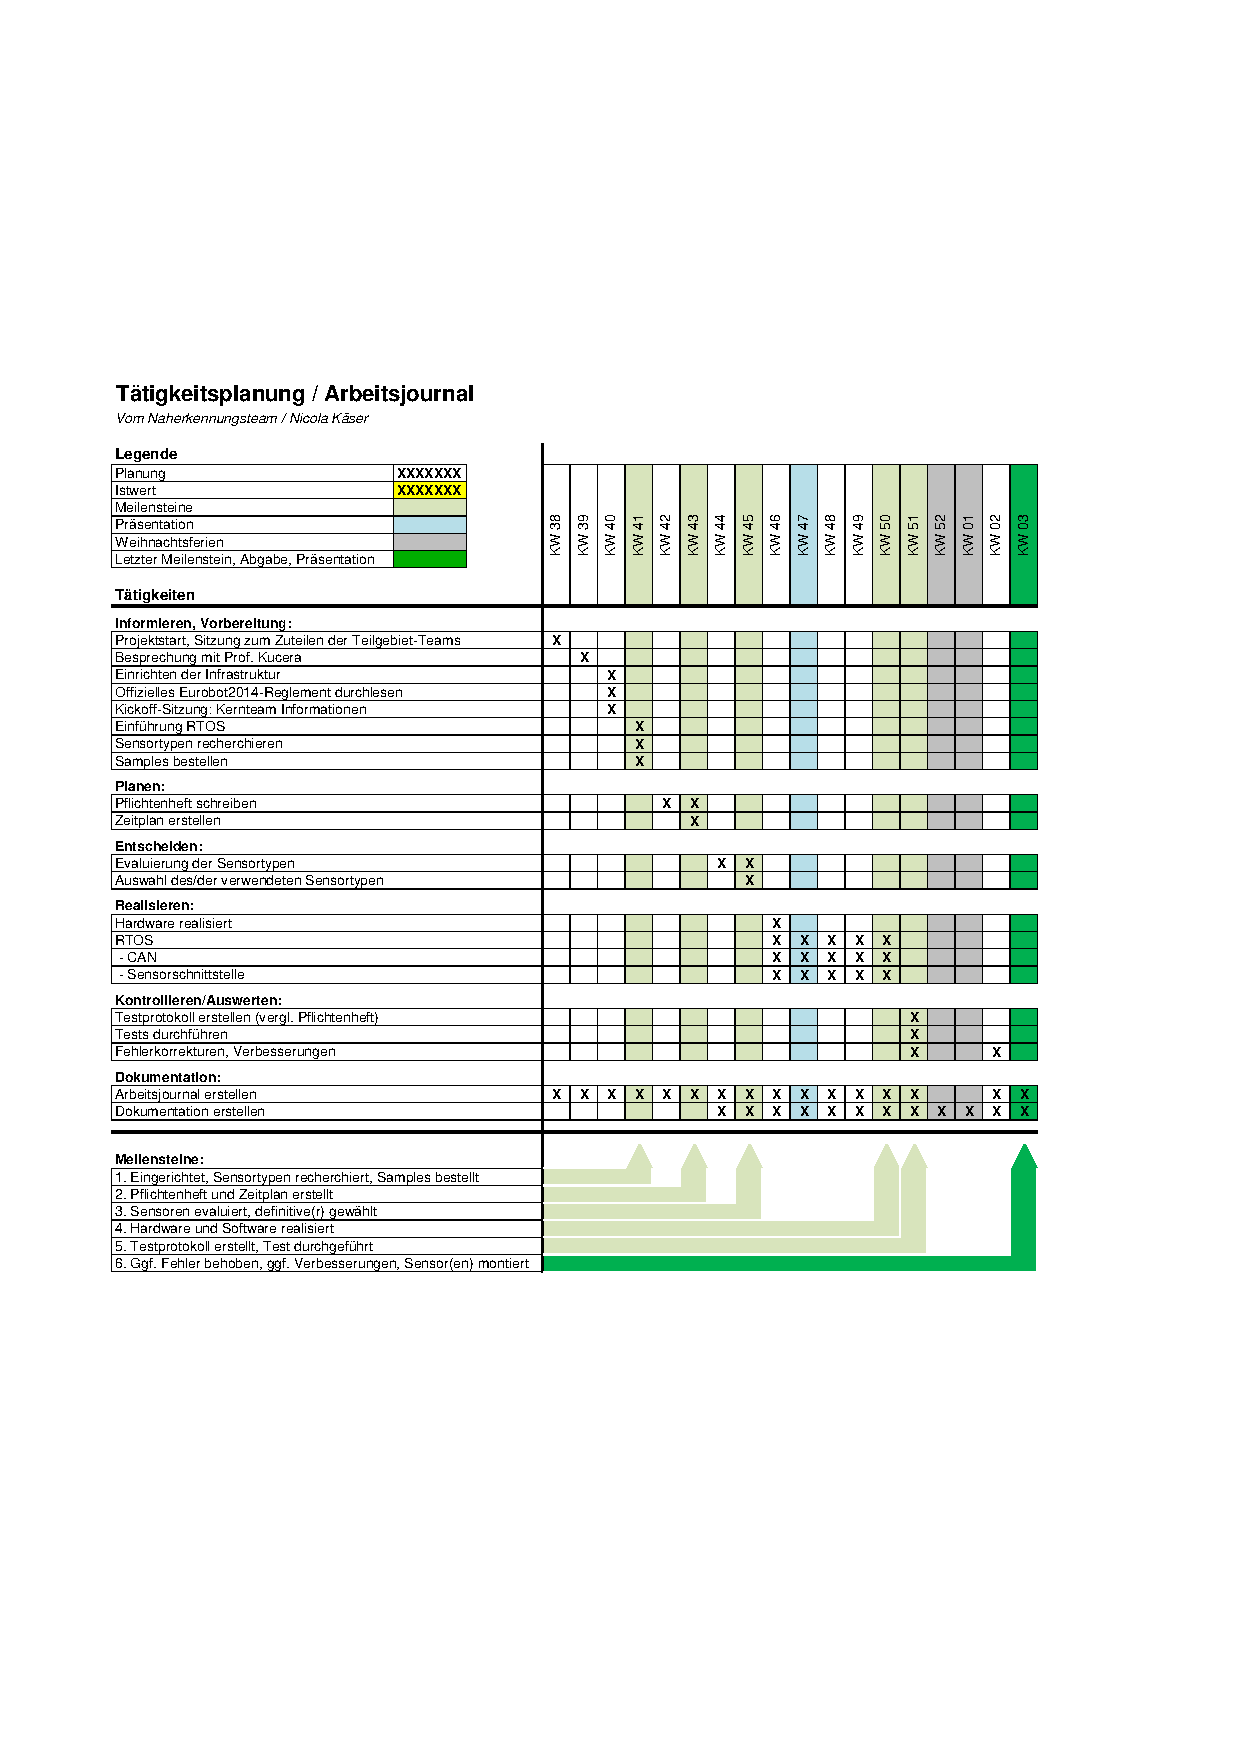
\includepdf[scale=1,pages=-]{appendix/anhangA_Zeitplan.pdf}
%
% Anhang B
\chapter{Bla}\label{ch:anhang_b}
\mypagenumbering
%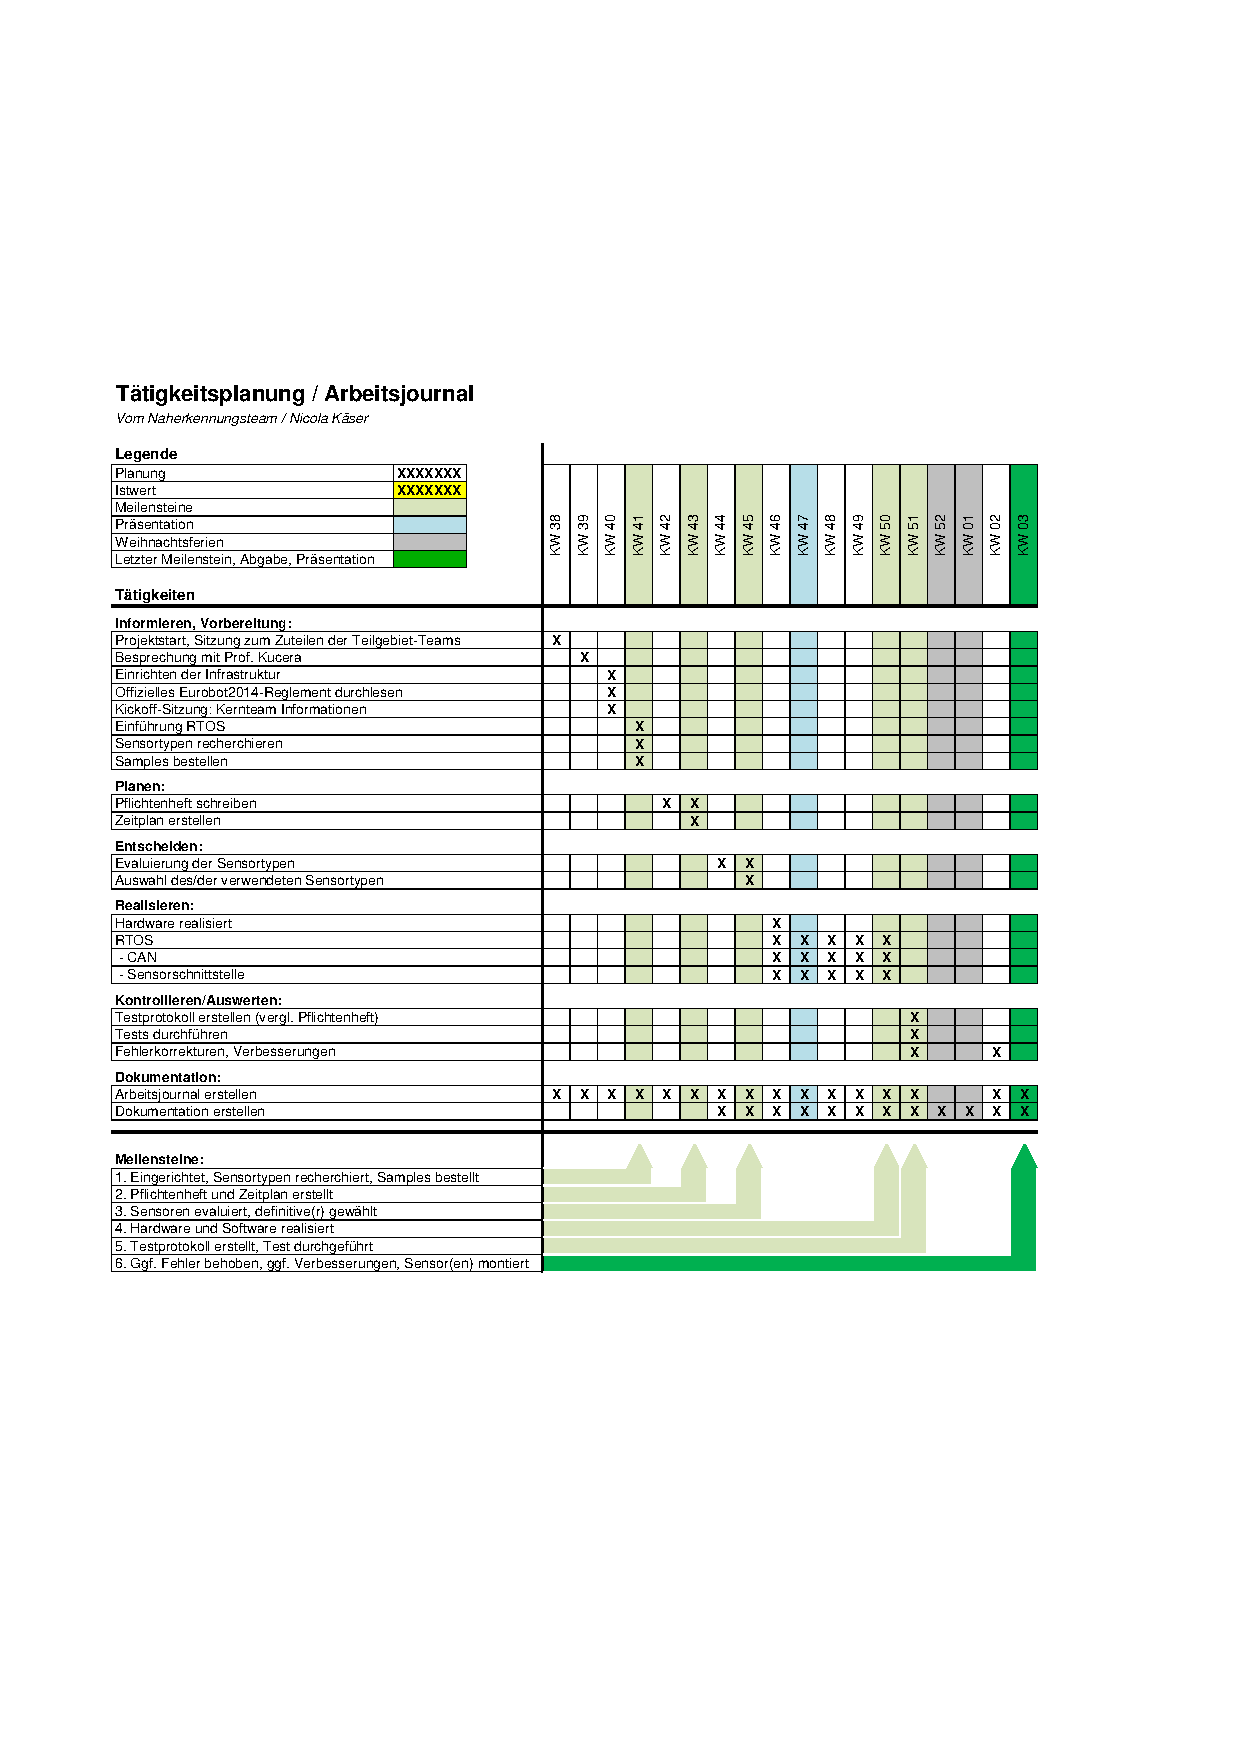
\includepdf[scale=1,pages=-]{appendix/anhangA_Zeitplan.pdf}
%
%
%
\end{document}